\documentclass{article}
\usepackage{graphicx}
\usepackage{caption}
\usepackage{hyperref}
\usepackage[margin=1in]{geometry}

\begin{document}

\section*{Graph Images}

Images are included relative to this file's location.

\begin{figure}[ht]
  \centering
  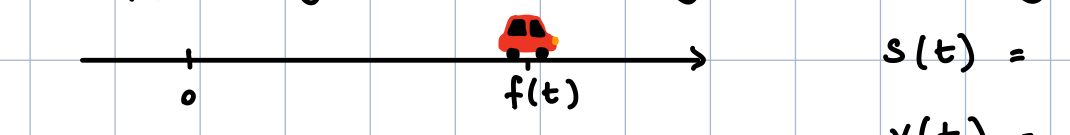
\includegraphics[width=0.8\textwidth]{graph_01_driving.png}
  \caption{Driving}
  \label{fig:driving}
\end{figure}

\begin{figure}[ht]
  \centering
  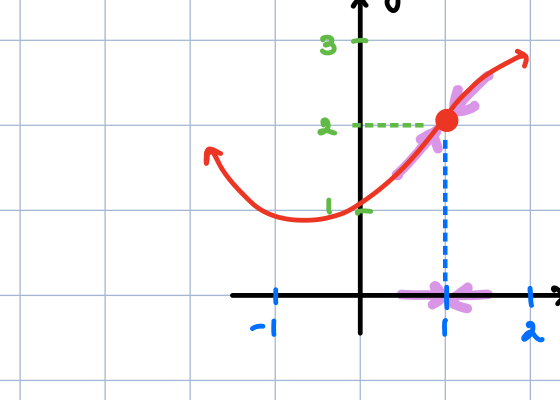
\includegraphics[width=0.8\textwidth]{graph_02_limit_continuous.png}
  \caption{Limit --- continuous}
  \label{fig:limit-continuous}
\end{figure}

\begin{figure}[ht]
  \centering
  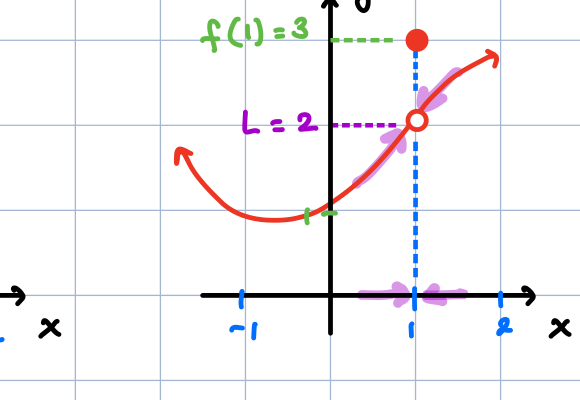
\includegraphics[width=0.8\textwidth]{graph_03_limit_hole_value_diff.png}
  \caption{Limit --- hole / value difference}
  \label{fig:limit-hole-diff}
\end{figure}

\begin{figure}[ht]
  \centering
  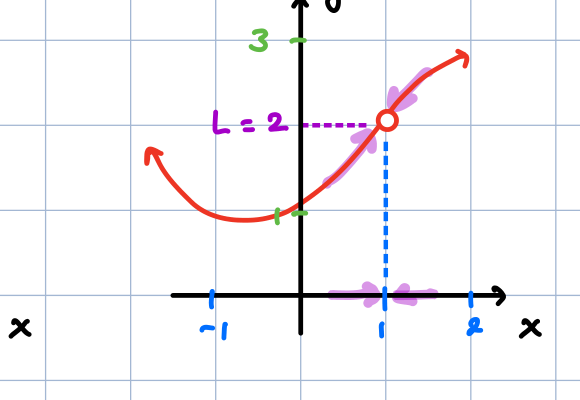
\includegraphics[width=0.8\textwidth]{graph_04_limit_hole.png}
  \caption{Limit --- hole}
  \label{fig:limit-hole}
\end{figure}

\begin{figure}[ht]
  \centering
  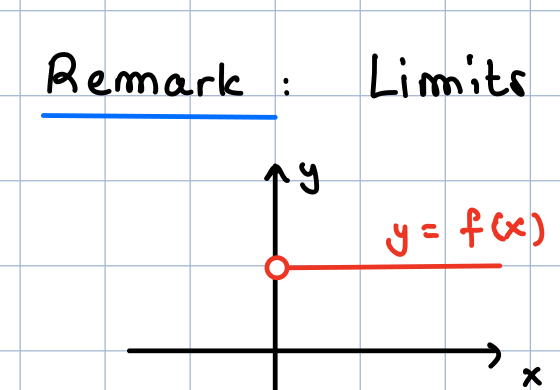
\includegraphics[width=0.8\textwidth]{graph_05_jump.png}
  \caption{Jump}
  \label{fig:jump}
\end{figure}

\begin{figure}[ht]
  \centering
  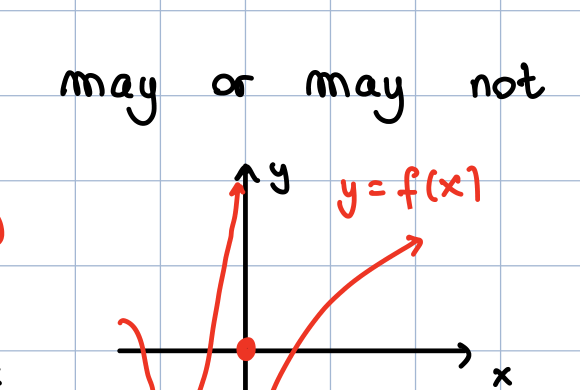
\includegraphics[width=0.8\textwidth]{graph_06_vertical_asymptote.png}
  \caption{Vertical asymptote}
  \label{fig:vertical-asymptote}
\end{figure}

\begin{figure}[ht]
  \centering
  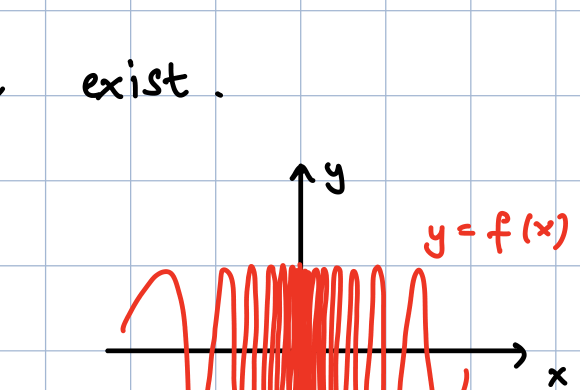
\includegraphics[width=0.8\textwidth]{graph_07_infinite_oscillation.png}
  \caption{Infinite oscillation}
  \label{fig:infinite-oscillation}
\end{figure}

\begin{figure}[ht]
  \centering
  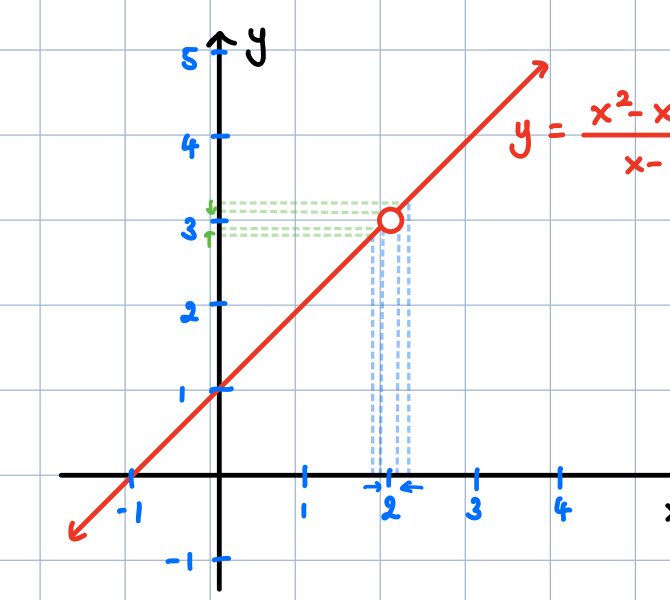
\includegraphics[width=0.8\textwidth]{graph_08_linear_with_hole.png}
  \caption{Linear with hole}
  \label{fig:linear-hole}
\end{figure}

\begin{figure}[ht]
  \centering
  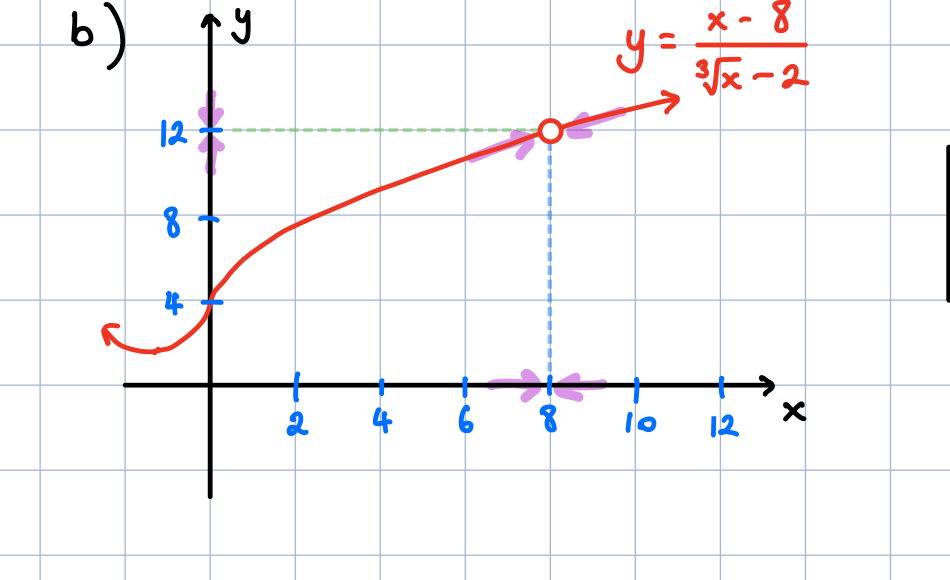
\includegraphics[width=0.8\textwidth]{graph_09_cube_root_curve.png}
  \caption{Cube root curve}
  \label{fig:cube-root}
\end{figure}

\vspace{1em}
For direct links to files:\\
\begin{itemize}
  \item \href{run:graph_01_driving.png}{Driving}
  \item \href{run:graph_02_limit_continuous.png}{Limit --- continuous}
  \item \href{run:graph_03_limit_hole_value_diff.png}{Limit --- hole / value difference}
  \item \href{run:graph_04_limit_hole.png}{Limit --- hole}
  \item \href{run:graph_05_jump.png}{Jump}
  \item \href{run:graph_06_vertical_asymptote.png}{Vertical asymptote}
  \item \href{run:graph_07_infinite_oscillation.png}{Infinite oscillation}
  \item \href{run:graph_08_linear_with_hole.png}{Linear with hole}
  \item \href{run:graph_09_cube_root_curve.png}{Cube root curve}
\end{itemize}

\end{document}
